\documentclass[border=4pt]{standalone}
\usepackage{tikz}
\usetikzlibrary{arrows}
\begin{document}
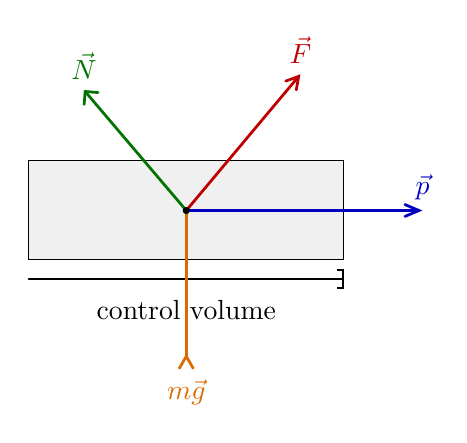
\begin{tikzpicture}[line cap=round]
  \draw[fill=gray!12] (0,0) rectangle (4,1.25);
  \draw[line width=.8pt,-{square bracket}] (0,-.25) -- (4,-.25)
    node[midway,below=4pt] {control volume};

  \draw[blue!75!black,line width=1pt,-{angle 45}]
    (2,.62) -- (5,.62) node[above] {$\vec p$};
  \draw[red!75!black,line width=1pt,-{angle 60}]
    (2,.62) -- (3.45,2.35) node[above] {$\vec F$};
  \draw[green!45!black,line width=1pt,-{angle 90}]
    (2,.62) -- (.7,2.15) node[above] {$\vec N$};
  \draw[orange!85!black,line width=1pt,-{angle 60 reversed}]
    (2,.62) -- (2,-1.4) node[below] {$m\vec g$};
  \fill (2,.62) circle (1.3pt);
\end{tikzpicture}
\end{document}
